\documentclass[conference]{IEEEtran}
\IEEEoverridecommandlockouts
% The preceding line is only needed to identify funding in the first footnote. If that is unneeded, please comment it out.
\usepackage{cite}
\usepackage{amsmath,amssymb,amsfonts}
\usepackage{algorithmic}
\usepackage{graphicx}
\usepackage{textcomp}
\usepackage{xcolor}

\usepackage{color, colortbl}
\usepackage{subcaption}
\usepackage{listings}
\usepackage{url}
\usepackage{epsfig}
\usepackage{multicol}


\def\BibTeX{{\rm B\kern-.05em{\sc i\kern-.025em b}\kern-.08em
    T\kern-.1667em\lower.7ex\hbox{E}\kern-.125emX}}

\definecolor{myred}{RGB}{248, 118, 109}
\definecolor{mygreen}{RGB}{0, 186, 56}
\definecolor{myblue}{RGB}{97, 156, 255}

\renewcommand{\arraystretch}{1.4}

\begin{document} 

%\title{DetGen: Data generation to bridge the "semantic gap" in network intrusion detection}
\title{Examining traffic micro-structures to improve model development}
%Dynamic Traffic Generation with Containerization for Machine Learning}

\maketitle

%\pagebreak
\begin{abstract}

We demonstrate how machine-learning-based network intrusion detection models can be validated and developed by probing models using traffic with specifically controlled micro-structures. We show our methodology by probing two published state-of-the-art models to find classification flaws and and understand misbehaviour. These models fail for input traffic with particular characteristics such as retransmissions or overly dispersed flow interarrival times. After we make simple corresponding model corrections, detection rates already improve between $2-4\%$.
% in response to these findings lead to immediate detection rate improvements between \textcolor{red}{...} percent.
We believe this shows promise for using tailored data with controllable and labelled characteristics to effectively improve model development in NID, a practice that helped model development significantly in several other areas of machine-learning.

\end{abstract}


\begin{IEEEkeywords}
Machine learning, traffic micro-structures, network intrusion detection
\end{IEEEkeywords} 	

%\pagebreak


\section{Introduction}

The model development process of machine-learning (ML) based network intrusion detection (NID) models usually ignores specific traffic characteristics and lacks the ability to extensively explore model failings. The main reason for this is likely the lack of precise datasets with specifically curated characteristics and corresponding information. In this paper, we demonstrate how the generation of traffic with controllable and labelled micro-structures enables researchers to probe a model and its reaction to various traffic phenomena to much greater detail in order to understand and develop the model's capabilities.

Machine-learning breakthroughs in other fields have often been reliant on a precise understanding of data structure and corresponding descriptive labelling to develop more suitable models.
%As an example, results in \textit{automatic speech recognition (ARS)} were not achieved by immediately training then state-of-the-art models on large annotated datasets. 
Initial models in \textit{automatic speech recognition (ASR)} for example were reliant on highly sanitised and structured speech snippets in order to isolate low-level structures such as phonemes or time-warping, before the understanding of these structures lead to the success of more layered models of feed-forward and recurrent neural networks and more recently fully end-to-end trained models. Lately, datasets that contain labelled specialised speech characteristics enable researchers to better understand ASR weak points such as emotional speech (RAVDESS), accents (Speech Accent Archive), or background noise (Urban Sound Dataset).

In a similar fashion, several approaches to enhance the way information is collected and presented have been successful in improving understanding between data and detection systems in different areas of information security. Virtual machine introspection monitors and analyses the runtime state of a system-level VM, and the inclusion of threat reports to create behavioural feature labels enriches the way executables are described \cite{smith2020mind}. Recently, data provenance tools aim to improve the representation of system executions \cite{barre2019mining} over traditional logs. 

However, such efforts have not been made in network intrusion detection yet, with the current quasi-benchmark datasets paying more attention to the inclusion of a wide variety of attacks rather than the close control and detailed documentation of the generated traffic. Data containing ground-truth on the traffic generation process to link observable structures with corresponding computational activities is rare, which has so far lead researchers to predominantly apply a number of ML-models to traffic datasets in the hope of edging out competitors. %In-depth analyses regarding which traffic characteristics lead to inaccurate predictions or cause a model to misbehave,
This overall lack of connection between the nature of intrusion detection data and the applied data-driven detection systems has been identified as a `semantic gap' by Paxson and Sommer \cite{sommer2010outside}, and is seen to be partly responsible for the lack of success machine-learning had in network intrusion detection. This claim has been supported and partly extended by Harang \cite{harang2014bridging} in 2014 and by Liu et al. in 2019 \cite{liu2019machine}.

In this work, we aim demonstrate the usefulness of the control and information on traffic micro-structures for model validation and development. We show the inspection of two state-of-the-art network intrusion detection models with specially generated traffic to identify model flaws, understand model behaviour better, and subsequently boost corresponding results. We hope to find new ways to improve model development in NID and increase the efficiency with which models can learn traffic micro-structures.


\subsection{Outline}

The remainder of the paper is organized as follows. Section \ref{Sec:Motivation} discusses the necessity for probing to validate and understand ML-models, and our methodology of using traffic micro-structure control for model probing. In Sections \ref{Sec:Improvedtrafficsep} and \ref{Sec:Refining} we demonstrate how to perform model probing and implement corresponding design improvements on two network intrusion detection models. Section \ref{Sec:Conclusion} 
concludes the results and discusses limitations of our work and directions for future work.

\section{Motivation and Methodology}\label{Sec:Motivation}

\subsection{Motivation}

Scientific machine learning model development requires both \textbf{model evaluation}, in which the overall predictive quality of a model is assessed to identify the best model, as well as \textbf{model validation}, in which the behaviour and limitations of a model is assessed through targeted \textbf{model probing}. Model validation is essential to understand how particular data structures are processed, and enables researchers to develop their models accordingly. Data generation tools for rapid model probing in other domains such as the \textit{What-If tool} \cite{wexler2019if} underline the importance of model validation.


\begin{figure}
\centering
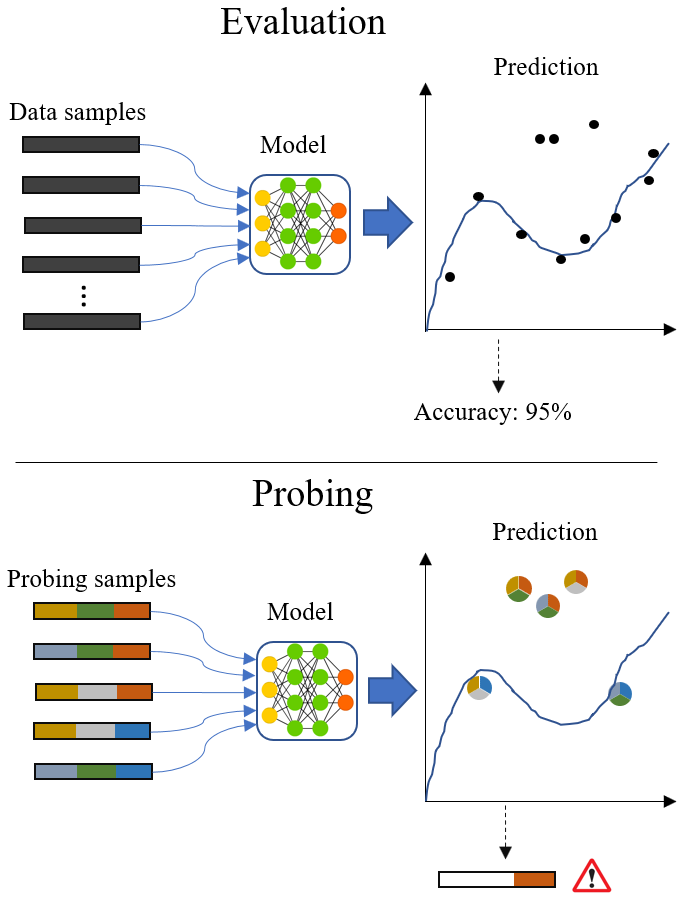
\includegraphics[width=0.45\textwidth]{images/Eva_Prob2.png}
\caption{Comparison between numerical model evaluation and model probing with specifically controlled data characteristics, indicated as colours.}\label{fig:Subspace_disp}
\end{figure}


We want to demonstrate how model validation can be performed for machine-learning-based network intrusion detection models such as traffic classifiers or anomaly-detection systems with the use of specifically generated traffic traces. We focus in particular on \textbf{traffic-micro-structures}, which we define as  short-term atomic, sequential or cumulative structures in the packet or flow metadata stream, compared to aggregate structures visible over longer periods. Differences in observable traffic micro-structures are driven through factors such as the particular communicational activity, the choice and implementation of the communication protocol as well as external effects such as network reliability or available computation resources. An analogue to this is speech, were influence factors such as accents or emotions can introduce structural characteristics to a conveyed message.


\subsection{Generating controllable traffic micro-structures}\label{Control}

We use a tool that generates various types of traffic with a fine-grained control over traffic shaping factors. In this work, we look traffic generated from scenarios that include regular HTTP communication, requests to an SQL-server, multi-host file-synchronisation, SQL-injection attacks, botnet traffic, as well as FTP-, SSH-, and SMTP-communication. The tool offers control over the following traffic shaping factors:


%The tool provides a set of 29 traffic scenarios to cover a variety of traffic types and offers control and if necessary randomisation of the following traffic shaping factors:

 
\paragraph{Performed task and application}
The conducted computational task and application ultimately drives the communication between computers, and thus hugely influences characteristics such as the direction of data transfer, packet rate, or the number of connections \cite{stober2013you}.


\paragraph{Application layer implementations}
Different implementations for TLS, HTTP, etc. can yield different channel prioritisation and can perform different handshakes.

\paragraph{Transferred data} 
The amount and content of transferred data influences the overall packet number, rate, and size such as shown by Biernacki \cite{biernacki2017analysis} for streaming services.


\paragraph{Caching/Repetition effects}
Tools like cookies, website caching, DNS caching, known hosts in SSH, etc. remove one or more information retrieval requests from the communication, which can lead to altered packet sequences and less connections being established \cite{fricker2012impact}.


\paragraph{Host level load}
Computational load (CPU, memory, I/O) on the host machine can affect the processing speed of incoming and outgoing traffic.

\paragraph{LAN and WAN congestion}
Low available bandwith, long RTTs, or packet loss can have a significant effect on TCP congestion control mechanisms, which in turn influence frame-sizes, IATs, window sizes, and the overall temporal characteristic of the sequence.

\vspace{0.2cm}

In this work, we focus mainly on influence from the factors \textit{a), b), f)} and partly \textit{c)}.


Labels that describe the respective setting for each factor are attached to each traffic sample after generation, thus enabling us to provide ground-truth information about the precise generation setting of individual samples. Traffic is generated in a virtual network along with virtual software switches, Ethernet links and routers. The communication is mostly performed in a client-server setting, however some settings such as multi-host file-synchronisation involve more hosts. 

%\textcolor{red}{labelling}

\subsection{Methodology}

Before the probing, we have to identify which types of characteristics the model should be probed on, and generate the corresponding data. We then train the model mainly on the datasets that is used for the general evaluation, but also attach a sufficient amount of the data dedicated for model probing to the training set. This is to ensure that the model is able to see and learn the structures in the probing data, even though the overall type of traffic in the probing data should be similar to the evaluation data to provide a consistent model.

After training and general evaluation, the model probing is done by feeding the model data samples with the desired descriptive labels, monitoring the output or behaviours in dependence of these labels, and comparing them to the expected output or behaviour. Since each traffic sample contains multiple descriptive labels, it is possible to monitor the model response to multiple characteristics in parallel.

%Containers communicate in a virtual network created with Mininet along with virtual software switches, Ethernet links, routers, and firewalls.


%Detgen is a container-based network traffic generation framework that \textcolor{red}{we} developed to enable repeatable, controllable, and informative network experiments. In contrast to the pool of programs running in a VM-setup, DetGen separates program executions and traffic capture into distinct containerised environments in order to shield the generated traffic from external influences and enable the fine-grained control of traffic shaping factors.

%Traffic is generated from a set of 29 scripted \textit{scenarios} setting such as HTTP server-client with various server implementations, file-synchronisation between several hosts, or malicious settings such as an SQL-injection attack with SQL-backend server. Each scenario consists of several sub-activities such as specific application actions (GET, POST, etc.) and input modes (content caching, wrong password, connection termination, etc.) as well as external influences (network congestion, host load, etc.)
%to strictly control major traffic shaping factors. %It offer researcher to modify and label the conducted activity from a variety of angles and randomisations. 
%Containers communicate in a virtual network created with Mininet along with virtual software switches, Ethernet links, routers, and firewalls.

%In the following experiments, we rely on DetGen to generate traffic data with corresponding micro-structure information labels.

%\section{Use-cases}

%\subsection{Impacts of ground-truth information on model understanding}

%Extensive ground-truth labels on different traffic influences as well as the ability to generate traffic with specific characteristics are arguably the most important contribution of the DetGen framework. We demonstrate their benefits for model-understanding and evaluation on two examples using a recent traffic classification model by Hwang et al. \cite{hwang2019lstm} and a highly regarded anomaly detection model by Casas et al. \cite{casas2012unsupervised}.


\section{Improved traffic separation for a classifier with congestion level information}\label{Sec:Improvedtrafficsep}


%Possible title: \textbf{Exploring the effect of rare events to model performance}
Our first example looks at how descriptive ground truth information on traffic characteristics can improve a traffic classification model through the analysis of data separation in dependence of different traffic features. For this, we use a recent traffic classification model by Hwang et al. \cite{hwang2019lstm} as an example, which aims at distinguishing various types of malicious activity from benign traffic. The model achieved some of the highest detection rates of packet-based classifiers in a recent survey \cite{tahaei2020rise}.
The model classifies connections on a packet-level using a \textit{Long-short-term memory} (LSTM) network \footnote{a deep learning design for sequential data}, and is claimed to achieve detection and false-positive (FP) rates of \textbf{99.7\%} and \textbf{0.03\%} respectively. 


We train a model on a set of different HTTP-activities in order to detect SQL-injections. Rather than providing an accurate and realistic detection setting, this example shows how traffic information can be linked to model failures and slumping performance. We use real-world HTTP-traffic from the \textit{CAIDA anonymized traffic traces} \cite{walsworth2015caida} as background traffic (85\% of connections) and add SQL-injection attack traffic (7.5\%) as well as different HTTP-activities for probing (7.5\%). In total, we use 50,000 connections for training the model, or slightly less than 2 million packets. 


\begin{figure}
\centering
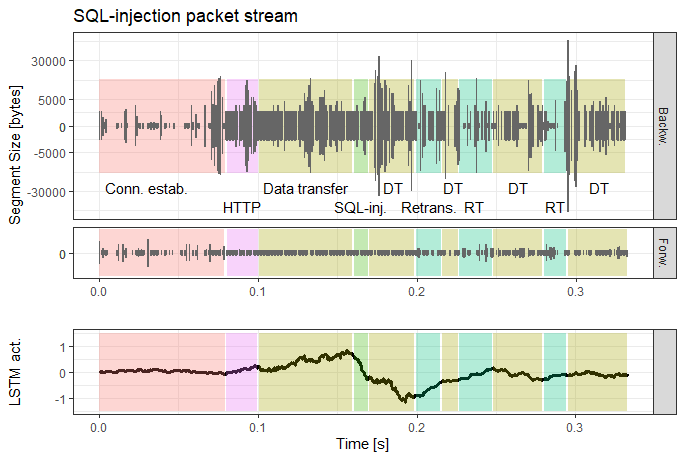
\includegraphics[width=0.5\textwidth]{images/LSTM_activation.png}
\caption{LSTM-output activation in dependence of connection phases. Depicted are packet segment streams and their respective sizes in the forward and backward direction, with different phases in the connection coloured and labelled. Below is the LSTM-ouput activation while processing the packet streams.}\label{fig:LSTM_act}
\end{figure}

The initially trained model performs relatively well, with an \textit{Area under curve} (AUC)-score\footnote{a measure describing the overall class separation of the model} of \textbf{0.981}, or a detection and false positive rate\footnote{tuned for the geometric mean} of \textbf{0.96\%} and \textbf{2.7\%}. However, these rates are still far from enabling operational deployment. Now suppose we want to improve these rates to both detect more SQL-injections and retain a lower false-positive rate.

We initially explore which type of connections are misclassified most often. For this, we perform a correlation analysis between the numeric or categoric labels available for the probing data, and the binary response whether the corresponding connection was misclassified. Unsurprisingly, the highest correlation to misclassification was measured for the conducted activity, with a particular attack scenario (19\% correlation) and connections with multiple GET-requests (11\% correlation) being confused most often. This was followed by the amount of simulated latency (12\% correlation), which we are now examining closer.



Fig. \ref{fig:LSTM_exp} depicts classification scores of connections in the probing data in dependence of the emulated network latency. The left panel depicts the scores for the initially trained model, which shows that while classification scores are well separated for lower congestion, increased latency in a connection leads to a narrowing of the classification scores, especially for SQL-injection traffic. Since there are no classification scores that reach far in the opposing area, we conclude that congestion simply makes the model lose predictive certainty. 
Increased latency can both increase variation in observed packet interarrival times (IATs), and lead to packet out-of-order arrivals and corresponding retransmission attempts. Both of these factors can decreases the overall sequential coherence for the model, i.e. that the LSTM-model loses context too quickly either due to increased IAT variation or during retransmission sequences. 


\begin{figure}
\centering
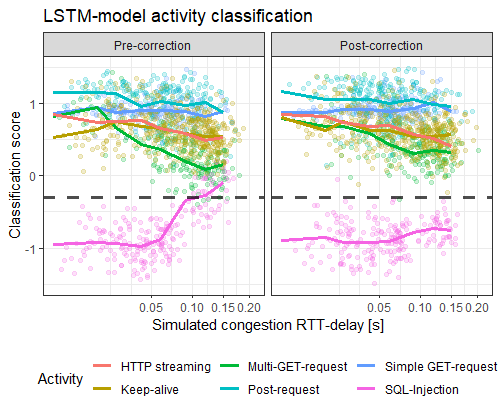
\includegraphics[width=0.5\textwidth]{images/LSTM_classi.png}
\caption{Scores for the LSTM-traffic classification model in dependence of simulated network congestion, along with the classification threshold. }\label{fig:LSTM_exp}
\end{figure}

To examine the exact effect of retransmission sequences on the model output, we generate two similar connections, where one connection is subject to moderate packet loss and reordering while the other is not. We then compare how the LSTM-output activation is affected by retransmission sequences. Fig. \ref{fig:LSTM_act} depicts the evolution the LSTM-output layer activation in dependence of difference connection phases. Initially the model begins to view the connection as benign when processing regular traffic, until the SQL-injection is performed. The model then quickly adjusts and provides a malicious classification after processing the injection phase and the subsequent data transfer. The negative output activation is however quickly depleted once the model processes a retransmission phase, and is afterwards not able to relate the still ongoing data transfer to the injection phase. When comparing this to the connection without retransmissions, we do not encounter this depletion effect, instead the negative activation persists after the injection phase.

We try to correct the existing model with a simple fix by excluding retransmission sequences from the model input data, both during training and classification. This leads to significantly better classification results during network latency, as visible in the right panel of Fig. \ref{fig:LSTM_exp}. SQL-injection scores are now far-less affected by congestion while scores for benign traffic are also less affected, albeit to a smaller degree.
The overall AUC-score for the model improves to \textbf{0.997} while tuned detection rates and false positives improved to \textbf{99.1\%} and \textbf{0.045\%}.



\section{Refining the notion of benign traffic for anomaly detection}\label{Sec:Refining}

Next, we show how ground-truth traffic information can help produce more coherent clusters and thus refine the benign traffic model in anomaly-detection. In particular, we will examine a 
simplified version of \textit{Kitsune} \cite{mirsky2018kitsune}, a recent deep learning anomaly-detection model based on stacked autoencoders. \textit{Kitsune's} AUC-scores surpassed those of other state-of-the-art methods for a variety of attacks, including various types of Botnet traffic and \textit{man-in-the-middle} attacks.

%for access attacks according to a survey by Nisioti et al. \cite{nisioti2018intrusion}.
The model takes connection packet streams as input, which are pushed through an artificial information bottleneck before reconstruction, which forces the model to learn and compress reoccurring traffic structures. The compressed connection representation is essentially a positional projection into a lower-dimensional vector space, where spatial boundaries around benign traffic can be drawn. For demonstration purposes, we use a widely-used clustering approach for anomaly-detection rather than \textit{Kitsune's} more complex ensemble method. 
%This allows us to project flows into a lower-dimensional vector space, where spatial boundaries around benign traffic can be drawn using clustering to identify anomalous traffic events. The model takes 102 flow summary statistics as input, which include features such as packet size and interarrival statistics, flag occurrencies, or number of flows in window. 
Here, anomalous outliers are detected using the Mahalanobis-distance of a projected connection from identified cluster centers. %The identified clusters therefore serve as structural enclosures of benign behaviour, with the cluster borders acting as separators to abnormal behaviours. 
Benign traffic should ideally be distributed evenly around the cluster centres to allow a tight borders and good separation from actual abnormal behaviour.

Unstructured datasets such as the CAIDA traffic traces assumably contain too much abnormal behaviour to train an anomaly-detection model, which is why we train the model on benign traffic from the CICIDS-17 \cite{sharafaldin2018toward} intrusion detection dataset (80\%). Again, we add 20\% probing traffic consists of HTTP, FTP, SSH, and SMTP communication, using a wide spectrum of settings for examination purposes. Attack data for the evaluation was again provided through the CICIDS-17 dataset, and includes access attacks such as SQL-injections or Brute-Forcing, as well as Mirai botnet traffic. We  train the model with in total 150,000 connections.

\subsection{Projection coherency evaluation}

\begin{table}
\centering
\begin{tabular}{p{0.8cm}|p{2.3cm}|p{1.5cm}|p{1.6cm}}
Label&\textbf{HTTP}&\textbf{File-Sync} & \textbf{Mirai-C\&C}\\ \hline 
\textbf{1}& Get-req. NGINX, low lat.&  Two hosts, low lat. & Command 1, low lat. \vspace{0.1cm} \\ \hline
Results:& \textcolor{myblue}{0.14}\space ,\space\space\textcolor{myred}{0.45} 
&\textcolor{myblue}{0.19}\space ,\space\space\textcolor{myred}{0.27} 
&\textcolor{myblue}{0.03}\space ,\space\space\textcolor{myred}{0.06}\\ \hline \hline
\textbf{2}&Multi-req. NGINX, low lat. & Four hosts, low lat. & Command 2, low lat.\\ \hline
Results:&\textcolor{myblue}{0.32}\space ,\space\space\textcolor{myred}{0.45} 
&\textcolor{myblue}{0.15}\space ,\space\space\textcolor{myred}{0.33} 
&\textcolor{myblue}{0.03}\space ,\space\space\textcolor{myred}{0.04}\\ \hline \hline
\textbf{3}& Post-req. Apache, high lat. &Two hosts, high lat. & Command 3, high lat.\\ \hline
Results:&\textcolor{myblue}{0.17}\space ,\space\space\textcolor{myred}{0.28} 
&\textcolor{myblue}{0.16}\space ,\space\space\textcolor{myred}{0.28} 
&\textcolor{myblue}{0.02}\space ,\space\space\textcolor{myred}{0.04}\\ \hline \hline
\textbf{4}& Multi-req. Apache, high lat. & Four hosts, high lat. & Command 4, high lat.\\ \hline
Results:&\textcolor{myblue}{0.53}\space ,\space\space\textcolor{myred}{2.51} 
&\textcolor{myblue}{0.71}\space ,\space\space\textcolor{myred}{1.31} 
&\textcolor{myblue}{0.03}\space ,\space\space\textcolor{myred}{0.05}\\ \hline \hline
\end{tabular}
\caption{Outline of the traffic settings for examining projection consistency. The numbers below each setting describe the measured Mahalanobis-distances (blue:average, red:maximal) for the corresponding projections.}\label{Tab:Dataset}
\end{table}

Like many approaches that generate representations of benign traffic for anomaly detection, \textit{Kitsune} projects traffic events into a vector-space where traffic clusters and similarities become more apparent. In order for the projection to accurately capture important traffic structures, this projection should be consistent, i.e. traffic events with similar origins and characteristics should be projected to similar positions rather than be dispersed throughout the vector space \cite{hou2017deep}.

%Verifying the projection consistency of a model is not straightforward as usually no or not enough ground-truth information about different traffic characteristics is available to asses if the model is projecting similar traffic to dissimilar positions, or if the traffic just bears some dissimilar characteristics.

To verify the models projection consistency, we generate traffic from near-identical conditions to provide certainty on the expected traffic similarities. We generate a small dataset that consists of HTTP-requests, file-synchronisation, and Botnet communication. For each of the three traffic types we fix four settings that vary in the performed activity and network latency, with the traffic shaping described in Section \ref{Control} being held constant within each setting except for small variations in the transmitted message or file. Table \ref{Tab:Dataset} summarises the traffic for each setting. 

We verify if traffic samples within each group are projected to similar areas by measuring the average and maximum Mahalanobis-distance to quantify the overall dispersion of the samples. The results are displayed in Table \ref{Tab:Dataset} and depicted in Fig. \ref{fig:Subspace_disp}. The first thing to notice is that the model projects samples from each group within the same cluster, thus confirming the capture of a coarse traffic structure. When looking at the traffic dispersion and the corresponding Mahalanobis-distance measurements, we notice that the \textit{multi-request HTTP} traffic as well as the \textit{file-synchronisation} between mutliple computers is much further dispersed than in the other settings, especially when exposed to more latency. We also find that the corresponding dimension, $x_3$, with the most projected dispersion seems to be the same for each of the four settings. This suggests that the cause for the dispersion is the same for the different traffic types. 

We now focus on the influence of input features on the projected positions exclusively in the $x_3$-direction. Here, we can again perform a simple correlation analysis between different the input feature values and the corresponding $x_3$-value. We observe that the arrival time of packet bears the most correlation (5.4\%) for the selected settings. We also see that this influence is concentrated primarily on connections that are opened shortly after a previous connection, with the temporal separation between these two connections apparently being the primary cause for the spread on the $x_3$-axis. The connection interarrival times are naturally an important feature for \textit{Kitsune} to detect attacks such as \textit{Man-in-the-Middle}, which could explain the weight this feature plays in the projection process.

%look at the the influence of the individual flow features on projected position, we notice that even slight differences in the IAT of the preceding and the subsequent flow impacts the projected position quite strongly, which is why only the settings that generate multiple flows are affected.


\begin{figure}
\centering
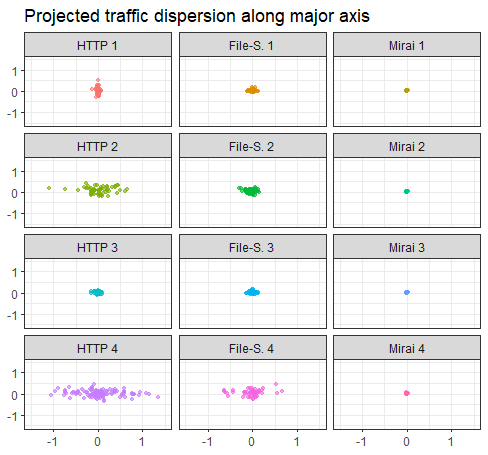
\includegraphics[width=0.5\textwidth]{images/traffic_dispersion.png}
\caption{Dispersion of projected traffic samples from each setting, plotted along the two most dispersed axes.}\label{fig:Subspace_disp}
\end{figure}


%at the effect of sudden connection terminations on an anomaly-detection model by Casas et al. \cite{casas2012unsupervised}. 

\subsection{Investigating individual cluster incoherences}


When examining false-positive and corresponding anomaly scores, we noticed that the model often classifies Brute-Force Web attacks as benign and some HTTP-traffic as anomalous. When examining the projected location of the corresponding connections, we see that most of this HTTP-traffic as well as the Brute-Force attack traffic lie near a particular cluster, depicted in Fig. \ref{fig:Subspace_projection}. A significant portion of traffic in that cluster seems to be spread significantly more across the cluster axis than the rest of the traffic in that cluster, leading to an inflated radius that partially encompasses Brute-Force traffic. 

When cross-examining the traffic in this cluster with the probing data, we see that HTTP-traffic with the label "Sudden termination" are distributed across the cluster axis in a similar fashion, also depicted in Fig. \ref{fig:Subspace_projection}, suggesting the conclusion that this type of traffic causes the inflated cluster radius. DetGen generates traffic with the label "Sudden termination" as half-open connections which were dropped by the server due to network failure. One defining characteristic of such connections are that they are not closed with a termination handshake using FIN-flags. To better capture this defining characteristics in the modelling process, we included an additional feature attached to the end of a packet sequence that indicates a proper termination with FIN-flags in the modelling process.
The newly trained model now projects "Sudden termination" connections into a different cluster, which leads to a far better cluster coherence. The detection rate on Brute-Force attack traffic could thus be improved from \textbf{89.7\%} to \textbf{94.1\%}.

\begin{figure}
\centering
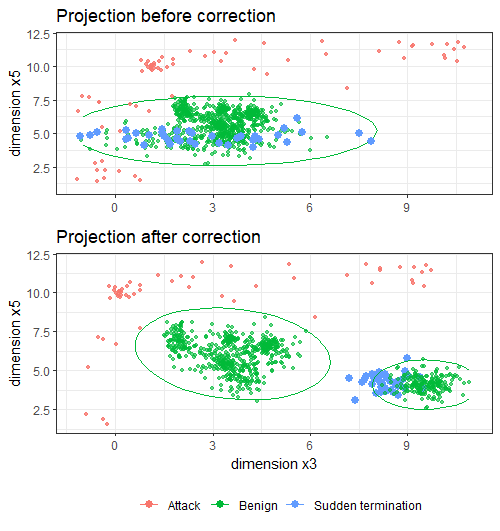
\includegraphics[width=0.5\textwidth]{images/Subspace_projection_new3.png}
\caption{Scores for the LSTM-traffic classification model in dependence of simulated network congestion, along with the classification threshold}\label{fig:Subspace_projection}
\end{figure}


\section{Conclusions}\label{Sec:Conclusion}

In this paper, demonstrated the impact of traffic generation with extensive micro-structure control as well as detailed corresponding documentation on researchers ability to evaluate and understand network intrusion detection models. We implemented and trained two state-of-the art detection models before extensively probing their behaviour and limitations when encountering different traffic types. 

By using HTTP-traffic with congestion settings, we were quickly able to identify the inability of an LSTM-based classifier to handle traffic with significant retransmission rates, which enabled us to improve the model accordingly and increase detection performance by more than $2\%$. Similarly, the examination of projection consistency of a subspace-clustering method using traffic with artificially similar characteristics revealed an overly high sensitivity to flow interarrival times, while cluster-coherence could be increased significantly by identifying half-open connections that were dropped because of network failure as the source of overly dispersed traffic projections. 

These results have encouraged us to perform more deep-going probing of data-driven network intrusion detection models. We believe that in combination with strong NID-dataset, extensive model validation and corresponding development with targeted traffic samples might hold the key to reduce false positives of detection models to an acceptable rate, as well as help models replicate detection rates in practical settings.

%It also shows that DetGen offers strong insights into traffic micro-structures and their effect on traffic models, and allows researchers to analyse the particular characteristics of events that lead to false-positives or model failure as well as their effect on model training.


%we proposed DetGen, a framework aimed at improving researchers understanding of traffic micro-structures and their respective effect on traffic models in order to close the \emph{semantic gap} described by Sommer and Paxson \cite{sommer2010outside}. DetGen allows reproducible traffic generation experiments that allow the control and monitoring different traffic shaping aspects while delivering data that is truthful to real-world structures. Our framework achieves this through containerised applications and corresponding process and traffic separation, meticulous attention to the corresponding generating activities and their facets, and the careful emulation and control of external effects. Currently, DetGen produces traffic for 29 different activities.

%We verified the improvements regarding reproducibility and traffic control of DetGen compared to traditional VM-setups in an experiment as well as the fidelity of the generated traffic to real-world characteristics in another experiment. Especially regarding the exclusion of background traffic and corresponding connection sequence structures, DetGen outperformed traditional setups significantly. In terms of traffic diversity, DetGen achieved significantly better results than current state-of-the-art NIDS-datasets.



%The major design advantages of this framework are the isolation of traffic scenarios into separate container arrangements, which allows the extension of new scenarios and detailed implementation of subscenarios as well as the capture of ground truth of the computational origins of individual traffic events. Furthermore, containerization enables the generation of traffic data at scale due to containers being light-weight and easily clonable.

%We verified the realism of the generated traffic and the corresponding ground truth information with two experiments, and demonstrated the usefulness of the framework in another experiment.
%Presently, our framework consists of 29 scenarios capable of producing benign and malicious network traffic. Several of these scenarios, such as the \emph{BitTorrent} or the \emph{Stepping-Stone} scenario, provide novel traffic data of protocols or behaviours that has not been widely available to researchers previously.


\subsection{Difficulties and limitations}

%DetGen is building network traffic datasets from a small-scale level up by coalescing traffic from different fine-grained activities together. 
While the control of traffic micro-structures helps to understand models that perform on a packet- or connection-level, it does not replicate realistic network-wide temporal structures, such as port usage distributions or long-term temporal activity. The probing of models operating on aggregated, behavioural, or long-term features is therefore not effective, and variation in these quantities would have to be statistically estimated from other real-world traffic beforehand to allow our framework to emulate such behaviour reliably. Other datasets such as UGR-16 use this approach to fuse real-world and synthetic traffic and are currently better suited to build models of large-scale traffic structures.

Furthermore, while controlling traffic shaping factors artificially helps at identifying the limits and weak points of a model, it can exaggerate some characteristics in unrealistic ways and thus both affect the training phase of a model as well as tilt the actual detection performance of a model in either direction. Additionally, the artificial randomisation of traffic shaping factors can currently not generate the traffic diversity encountered in real-life traffic and thus only aid at exploring model limits extensively. The lack of realistic traffic heterogeneity however is at the moment significantly more pronounced in commonly used network intrusion datasets such as the CICIDS-17 dataset, where the vast majority of successful FTP-transfers consist of a client downloading a single text file that contains the Wikipedia page for ‘Encryption’.

%We paid meticulous attention to enable control over as many traffic impact factors as possible. However, DetGen is currently only offering insufficient control over underlying application-layer implementations such as TLS 1.3 vs 1.2. In theory, it should be unproblematic to provide containers with different implementations for each scenario to provide this control. However we faced difficulties to compile containers in a suitable manner and are currently investigating, how to improve DetGen on this shortcoming.

%Working with Docker containers can sometimes complicate the implementation of individual scenarios compared to working with VMs. Although several applications are officially maintained Docker containers that are free from major errors, many do not. For instance, in the \textit{BitTorrent} scenario, most common command line tools, such as \texttt{mktorrent}, \texttt{ctorrent} and \texttt{buildtorrent}, failed to actually produce functioning torrent files from within a container due to Docker's union filesystem. Furthermore, due to the unique way in which we are using these software packages, unusual configuration settings are sometimes needed. %As such, many 

%Lastly, capturing \texttt{.pcap}-files from each container can quickly exceed available disc space when generating traffic at scale. Depending on specific research requirements, it is advizable to add filtering or feature extraction commands to the scenario execution scripts to enable traffic preprocessing in real-time.




%We are grateful for our ongoing collaboration with our industry partners  on this topic area, who provided both ongoing support and guidance to this work. Discussions with them have helped reinforce the need for a better evaluation and understanding of the possibilities that new intelligent tools can provide.

%Full funding sources after currently blinded.

\bibliographystyle{abbrv}
 
\bibliography{../DetGen_ext}

%\appendix


\end{document}
